\documentclass{article}
\usepackage{graphicx}
\usepackage{epstopdf}
\usepackage{url}
\bibliographystyle{unsrt}
\title{Improving parallelism for interactive realtime workloads\\ \vspace{1ex} Project proposal}
\author{Kjetil Raaen}

\setlength{\parskip} {1ex plus 0.5ex minus 0.2ex}
\setlength{\parindent}{0pt}

\begin{document}
\maketitle

\section{Introduction}
\label{intro}
Software developers have gotten used to exponential growth in computing power over the last few decades. This growth has led to a long series of innovations that, in
many ways, have changed the world. The exponential growth of circuit
complexity was first described by Gordon Moore~\cite{moore} while
working on early integrated circuits, and has continued since. One
common misunderstanding of Moore's law is that it describes an
exponential growth in performance. The paper only refers to growth in
complexity. This distinction is important; translating increased
transistor count to increased actual performance is
difficult. Recently, the growth in single-threaded performance has
more or less leveled off. Now, most performance gains
are based on increasing the number of processor cores in a chip\cite{dally}.

Utilizing these cores requires deep changes in how we make the
software. Amdahl's law~\cite{amdahl} states that the speedup achieved
by parallel processing is limited by the time needed for the
sequential fraction of the program. One of the main challenges to continued performance improvements is to reduce
this sequential fraction. Work on this problem has been ongoing for a
long time, but it is mostly focusing on batch processing tasks.
%%Her skulle jeg gjerne ha noen referanser, men det er jo så mange
%%eksempler og velge mellom. Finnes det en oversikt?

In contrast, modern computing consists of a range of tasks that are far
from bulk, or batch, number crunching. Interactive applications
require fast response times while still requiring a large amount of
calculations. This requirement is particularly important in
certain games~\cite{claypool++-2006}. Computer games are increasing rapidly in complexity and
processing requirements. Current Massively Multi-player On-line games (commonly refered to as "MMOs")
allow about a hundred people to congregate in one area. Simulation of
interactions between these players require large amounts of
processing. In the future, this number might be much greater, and the
simulation will be more detailed and sophisticated. To make this
situation acceptable to the players, the simulation will have to be
updated approximately every 100ms. Which means that developers have to
deal with deadlines as well as processing requirements.
%ref Mark Claypool~\cite{claypool++-2006} ... si litt mer om total
%opplevd latency for forskjellige spilltyper.  Slutter brått?
%Avrunding?  hardcore vs casual players...

\section{Areas of interest}
Games and other interactive multimedia applications have mostly been
designed using a single thread, with some specific workloads offloaded
to other threads. Under the current industry paradigm a multi-player game typically
consists of multiple clients connecting to a server, with only loose coupling between multiple servers.


This thesis will challenge the current paradigm by investigating how interactive multimedia applications
can be distributed to multiple threads and even multiple machines in a cluster.
The vision is an environment where workloads can be distributed freely among any number of nodes in a
server cluster as well as utilizing spare resources among any of the client computers, while still maintaining
a consistent state. This last is much more difficult in pure peer-to-peer approaches, where none of the nodes can be trusted.

%break down barriers 
%Parallel computing in a heterogeneous environment

\subsection {Distributing workloads across cores in a shared memory system}
The most obvious and perhaps simplest approach to distributing
workloads is using multiple threads in a single, shared-memory
computer, where all processing units are identical general purpose CPUs. The tool support for this is already good. Libraries
like Java's ThreadPoolExecutor~\cite{threadpool} handles most
implementation details, so developers can focus on algorithms. Such tools
make this an ideal testbed for experiments to find out how much code in
a given algorithm is serial, as well as what can be parallelized.

\subsection {Distributing workloads in heterogeneous multicore architectures}
Traditionally, servers have used identical general purpose CPUs for all tasks. Recently hardware manufacturers have moved
towards more heterogeneous architectures. The currently most relevant such system is Nvidia Tesla ~\cite{tesla}. This system
is based on graphics processing units adapted for scientific or simulation workloads. Utilizing these resources for interactive simulations is another area of interest in this thesis.

\subsection {Distributing workloads in server clusters}
Another area of focus, is to study how
workloads can be distributed across networks to separate
computers. This introduces network communication issues as well as
state coherence issues not present in the shared memory case. Tool
support is available for this situation too, but these are not as mature as for
the shared memory case. The most famous example of tools for this
environment is the Beowulf project~\cite{beowulf} though its focus is on bulk processing rather
than interactive or realtime workloads, it is still a good starting point.

%Games middleware?

\subsection {Offloading workloads to client computers }
\label{sec:offloadtoclients}
Many of the environments where interactive workloads are run, are
based on a client-server model. In the traditional MMO model the server has handled gameplay logic
 and any other task that is relevant to the rules of the game. This includes collision in 3d space
 as well as other heavy computational tasks. An  interesting area of focus is offloading some of
 this work to the clients. The same multiprocessing issues are
relevant here as in the cases described above. The issues are however, more complicated In addition
to these problems, using clients for computation leads to security
issues, since client computers can not be trusted in regular
circumstances. There is potential for developing a protocol that
allows us to trust client computers sufficiently to perform some
calculations. However it must be instigated under which situations is cost effective.

\subsection {Cloud computing in multimedia applications }
%Finne sitat som beskriver cloud computing?
Cloud computing has become increasingly popular for many applications
recently. Office applications, video and mail are all placed in the
cloud. Cloud services currently have a very high response time.
While this is acceptable for video services such as Youtube,
it becomes an annoyance in office applications that need some responsiveness, such as Google Docs, and is unacceptable for most games. It is therefore highly relevant to find out if this is due to a fundamental issue with the cloud technology, or if there are ways to get around this problem.
In this work we seek to investigate how we can overcome the response time limitations and make cloud services
viable for interactive realtime applications such as games.

\section{NITH Project integration}
This work will be funded by NITH, which has a BSC programme in game
programming as well as in game design. NITH is currently building a
group of researchers in different areas of game development to support
these programmes. There is currently one researcher working on user
interaction design in games, for support in tasks where  game
design requirements are relevant for the technical research. These
questions include: "How low does the latency need to be to satisfy the
players?", "What sort of interactions between players are relevant?"
and "Which interactions have to be transactional?"

Another research field at NITH that this work will integrate well
with is mobile phones. Mobile phones create a whole new area of
interest within parallel computing. Phones have less processing power
than traditional clients for interactive applications (i.e. PCs and
game consoles) so there might be a need for servers to take over more
of the work traditionally assigned to clients. On the other hand, it
is likely that phones will grow in processing power significantly in
the near future, and the phones can be used as worker nodes for the
server cluster as described for traditional clients
in~\ref{sec:offloadtoclients}.


\section{MPG Project integration}
The Media performance group (MPG) at Simula Research Laboratory (SRL)
investigates the means of overcoming or evading inhibitors for the use
of time-dependent digital media in distributed systems. The department
finds solutions by exploring, understanding and improving on a
particular inhibitor in an application context. Improvements are found
in better operating systems mechanisms, programming tools, protocols,
distributed architectures, digital media formats or a better
understanding of people's perception of media in a context. MPG
applies a multimedia systems approach, whereby successful research
leads to quantifiable improvements and success is proven
experimentally. The essential results of the research are algorithms,
methods, tools or prototypes that provide solutions for overcoming a
particular set of challenges in using time-dependent digital media in
distributed systems that are practical and realistic today or in the
near future.

The work described in this document is well attuned with the goals and
methods of MPG. The aims of provideing better support for
time-dependent tasks by developing strategies for parallel execution
with soft guarantees for timely delivery is especially comaptible with
the Parallel Processing Graph Framework (P2G) project who aims to
provide a complete solution for parallelization of real-time workloads
among heterogeneous architectures and networked nodes.


\section{Goals}
Achieving verifiable and quantifiable results by implementing and testing in prototype environments will be considered a priority. 

\subsection{Reduction in serial code fraction}
The foundation for any parallelization of algorithms will, according to
Amdahl's law always be reduction of the required serial fraction of
the code, hence this will be the initial goal of the thesis. We will also investigate how varying degrees of interdependence between actors influence latency and playability.

\subsection{Distribution of load}
When the workload is sufficiently parallel, the next goal is to move
from shared memory architectures to progressively more loosely coupled
nodes and towards heterogeneous architectures. 

\section{Applied method}
To reap the full benefit of parallel processing in interactive multimedia
applications a thorough analysis of the area of work is required. As
the most promising areas of effort reveal themselves, implementation
and subsequent testing will be required.  Following are the steps
required to complete this project:

\begin{enumerate}
   \item{}\textit{Analysis of application areas}\\
     A search and
     analysis will be performed with the goal of charting the most
     rewarding areas of improving parallelization and distributing
     work.
   \item{}\textit{Experiment designs}\\
     Promising areas found in the analysis will lead to the design of
     experimental systems.
   \item{}\textit{Implementation}\\
     The experimental designs will be implemented, and relevant tests
     will be run to collect data.
   \item{}\textit{Data analysis}\\
     The collected data will be analyzed.
   \item{}\textit{Compilation of results}\\
     The results of the data analysis, and the conclusions that can be
     drawn, will be compiled and presented in the thesis.
\end{enumerate} 
\section{Schedule}


\begin{enumerate}
%\begin{figure}
%\centering
%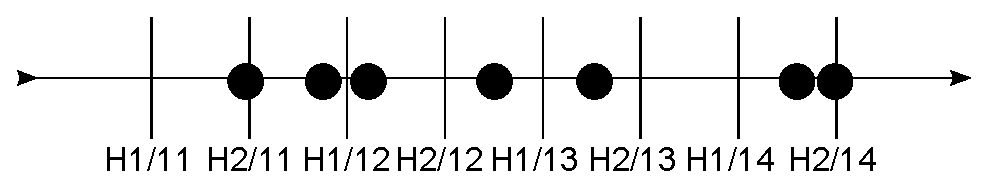
\includegraphics[width=10cm]{timeline.eps}
%\end{figure}

   \item{}\textit{10.2011}\\
   Demo paper describing the ideas and preliminary
   results. (Done: A demonstration of a lockless, reduced atomicity state model server. )
   \item{}\textit{12.2011}\\
   All mandatory courses completed.
   \item{}\textit{03.2012}\\
   Finished demonstration framework for a massive, realtime, parallel server.
   \item{}\textit{04.2012}\\
   Publish conference paper based on ideas from the LEARS demostration.
   \item{}\textit{06.2012}\\
   Extending the framework to shared memory clusters, publish paper based on results.
   \item{}\textit{06.2012}\\
   Third semester checkpoint.
   \item{}\textit{12.2013}\\
   Publish conference paper on peer-to-peer mesh network investigations.
   \item{}\textit{12.2013}\\
   Publish journal paper with the major results of the thesis.
   \item{}\textit{10.2014}\\
   Compilation of thesis finished.
   \item{}\textit{12.2014}\\
   Defence of thesis.

\end{enumerate}


\bibliography{pb}

\end{document}

